\chapter{The Large Hadron Collider and the ATLAS experiment}
\label{chap:ATLASdetector}

\chapterquote{Very inspiring quote}
{Very inspiring quote author}

%% LHC and ATLAS introduction
\section{The \LHC}
\label{sec:LHC}

The massive fruit of labour, decades in the making from the hundreds of institutions which make up CERN, lies hidden 100 meters below the surface of the Switzerland-France border. Sandwiched between Geneva and the Jura Mountains is a 27 km ring of superconducting magnets and radio-frequency (RF) cavities, which bend and accelerate particles to 0.999999991$c$. Mathematically, this is approximately 3 metres per second slower than the speed of light. This remarkable achievement is none other than the Large Hadron Collider (LHC). The LHC lives up to its name; it is the largest machine built by humankind, and unsurprisingly the most powerful high-energy particle collider in the world. The four main interaction points around the ring where particles collide mark the four main experiments: ATLAS, CMS, LHCb, and ALICE. The former two are general purpose detectors with a similar goal: to precisely study the Standard Model and to search for evidence of new physics. The latter two have specialized purposes. LHCb is dedicated to probing physics involving b-hadrons in pp collisions, and ALICE’s aim is to shed light on the physics of the quark-gluon plasma by investigating heavy-ion collisions. 

Prior to the injection into the LHC, the protons first pass through a series of smaller machines which boost them to higher and higher energy. The first in the chain is LINAC2, a linear accelerator that spouts protons (the source of which is hydrogen atoms with electrons stripped away) at \unit{50}{\MeV}. Next the protons are piped into the Proton Synchrotron Booster, the Proton Synchrotron, and finally into the Super Proton Synchrotron \todo{Give more details about each of these steps}. Through this chain the protons get boosted to \unit{1.4}{\GeV} by the PSB, then further to \unit{25}{\GeV} by the PS, to a final \unit{450}{\GeV} by the SPS before entering the LHC. Inside the pipes of the LHC, the protons take a short 20 minutes to reach \unit{6.5}{\TeV}. 

\begin{figure}
  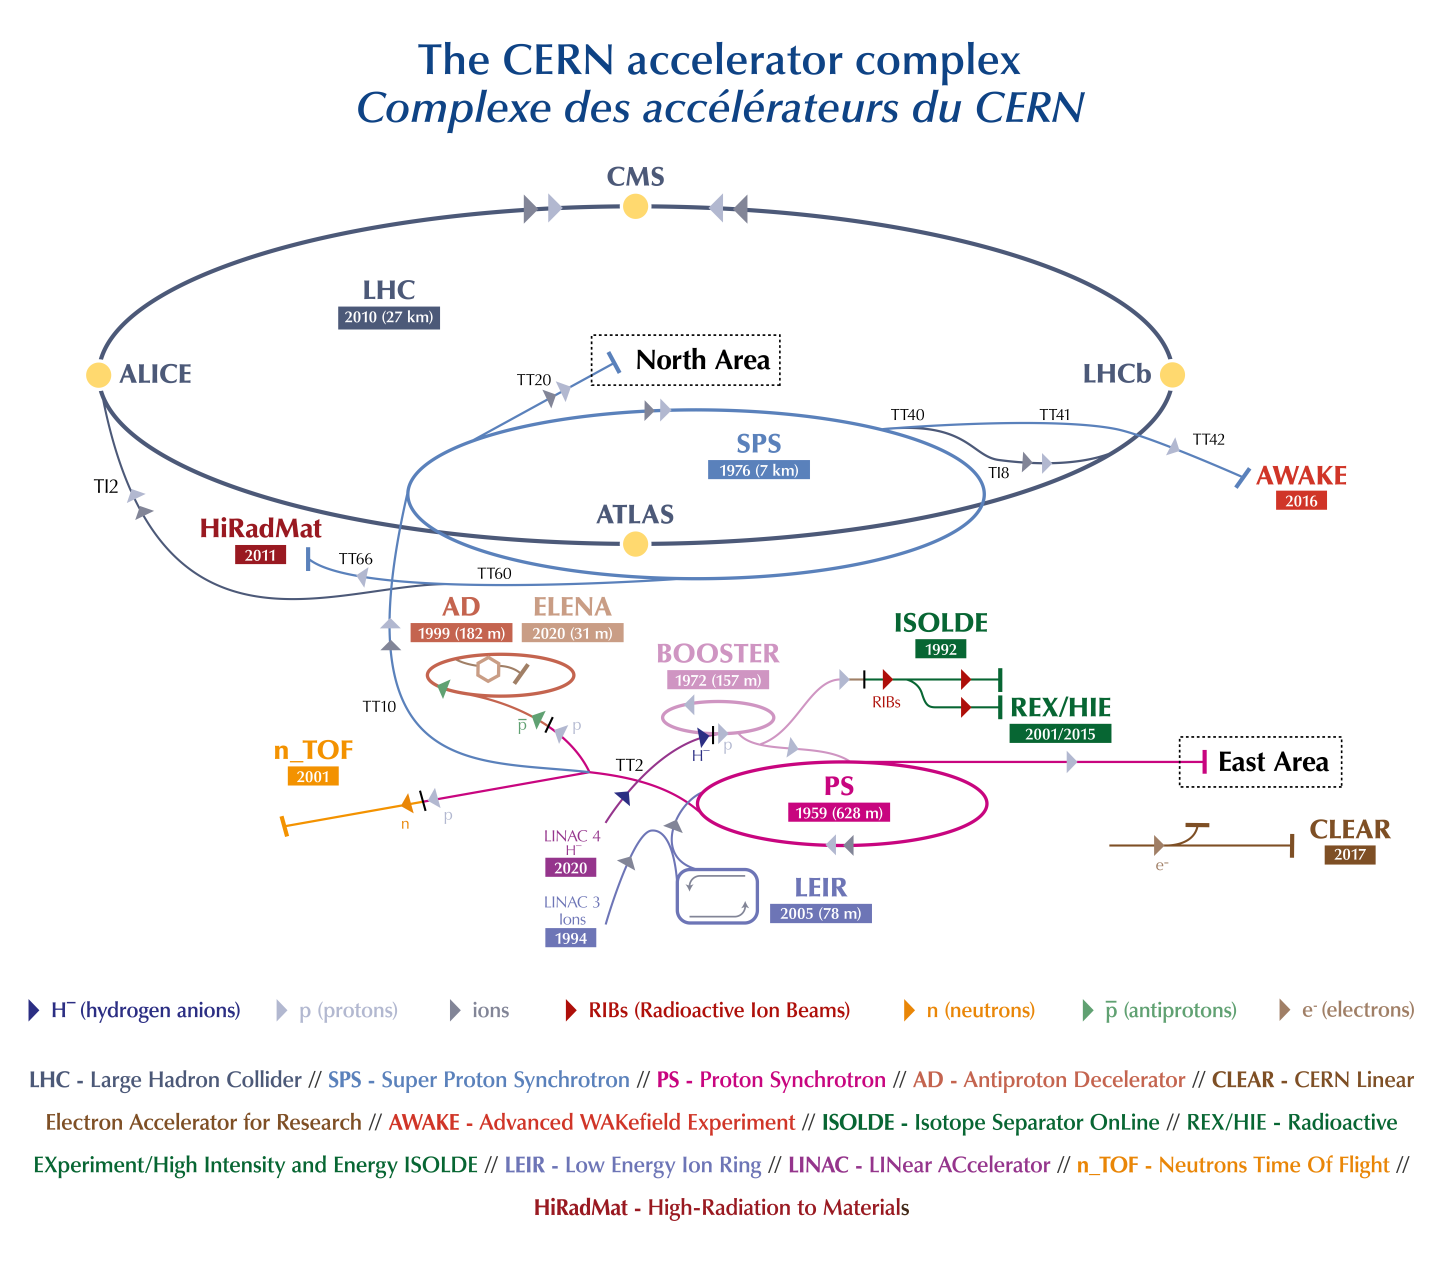
\includegraphics[width=\mediumfigwidth]{Figures/LHC/CernAcceleratorComplex.png}
  \caption[The \CERN accelerator complex]%
  {The CERN accelerator complex, where the LHC is the largest ring. The four main collision points corresponding to the main experiments are dotted in yellow.}
  \label{fig:CERNComplex}
\end{figure}

The impressive feat of accelerating particles is made possible through the use of radio-frequency cavities. The idea was first crafted by the young Rolf Wideröe \cite{vretenar2012radio} for his PhD thesis and later caught the eye of the brilliant E. Lawrence, recipient of the Nobel Prize in Physics in 1939 for the invention of the cyclotron. RF cavities are round chambers along the beam. A voltage generator generate a voltage which oscillates at \unit{400}{\mega\hertz}, inducing an electric field inside the RF cavity. As particles pass through they experience the force of the field and are accelerated along the beam pipe. In total the LHC uses 8 RF cavities per beam (so 16 in total), with each cavity capable of delivering a 2 megavolts (MV). Protons travelling through the cavity increase their energy to 14 times the injection amount, from 450 GeV to 6.5 TeV. Once protons get up to speed, a proton that has perfect timing will stay put, while protons that arrive slightly earlier/later will be accelerated/decelerate. The result is a beam of protons sorted into smaller segments of proton bunches. The LHC produces two such proton beams, one circulating clockwise and the other counterclockwise. 

An important key concept in particle physics is luminosity. It is a factor that relates the cross-section to the number of event per second, written as follows:
$$\luminosity=\dfrac{1}{\sigma}\cdot\dfrac{dN}{dt}$$
where \luminosity is the luminosity, $N$ is the number of events, and $\sigma$ is the production cross section. The dimension of luminosity is events per unit time and unit area \unit{}{\cm\rpsquared}\unit{}{\second\rp}.

There are two properties used to describe a particle beam: its \todo{write more about this} emittance $\epsilon$, and its $\beta$ function. The emittance can be thought of as the area occupied by the particle beam in the position momentum plane. A lower emittance means the distance between particles and the difference in momentum between the particles are small. The cross sectional sizes of the beam $\sigma_i$ ($i=x,y$) are written as 
$$\sigma_i=\sqrt{\dfrac{\beta_i\cdot\epsilon_i}{\pi}}$$ The beams are assumed to be Gaussian distributed, meaning that in collisions, the centres of the beams contribute most while the edges have minimal impact. Following this the luminosity is
$$\luminosity=\dfrac{N_1N_2f_{rev}N_b}{2\pi\Sigma_x\Sigma_y}$$
where $N_1$ and $N_2$ are the number of particles for each bunch, $N_b$ is the number of bunches, $f$ is the revolution frequency, and $\Sigma_x,\Sigma_y$ represent the \unsure[]{Read more about this!} convolution of the beam sizes. They can be expressed as
$$\Sigma_x=\sqrt{\sigma_{x1}^2+\sigma_{x2}^2}, \quad \Sigma_y=\sqrt{\sigma_{y1}^2+\sigma_{y2}^2}.$$
Assuming that the beam sizes are identical and round, $\sigma_{x1}=\sigma_{x2}=\sigma_{y1}=\sigma_{y2}$, and the luminosity becomes
$$\luminosity=\dfrac{N_1N_2f_{rev}N_b}{4\pi\sigma^2}=\dfrac{N_1N_2f_{rev}N_b\gamma}{4\pi\epsilon_N\beta^*}.$$

When proton beams cross at the LHC, there are many collisions which occur other than the hard-scatter of interest. While increasing the number of particles per bunch increases the likelihood of a rare interaction, it also increases the pile-up of multiple interactions. Pile-up, denoted as $\mu$, is one of the biggest obstacles for LHC experiments; the more there is, the more difficult it becomes to disentangle the events of interest from the sea of low energy collision. It is, however, an inevitable consequence that accompanies increasing the instantaneous luminosity \todo{Write more about why int. lumi. is wanted to be high}. The contribution to pile-up events can be separated into two main categories: 
\begin{itemize}
  \item In-time pile-up refers to simultaneous proton-proton collisions occurring in the same bunch crossing as the hard scatter of interest;
  \item Out-of-time pile-up is the overlay of events from neighbouring bunches which contaminate signal events, attributed to detector electronics latency.
\end{itemize}
There are also less-substantial contributions from the cavern background, beam halo events, and beam gas events. The cavern background is the cloud of gas that floods the LHC cavern during operation. Beam halo events are from when the proton beam interacts with the collimating instrumentation, and the beam gas events describe interactions between the beam and the residual gas in the beam pipe. 

The \LHC was originally designed to reach a peak instantaneous luminosity and average pile-up of \unit{$10^{34}$}{\rpsquare{\cm}\reciprocal{\second}}\todo{Citation?} and $\langle\mu\rangle=19$ respectively. 

\begin{figure}
  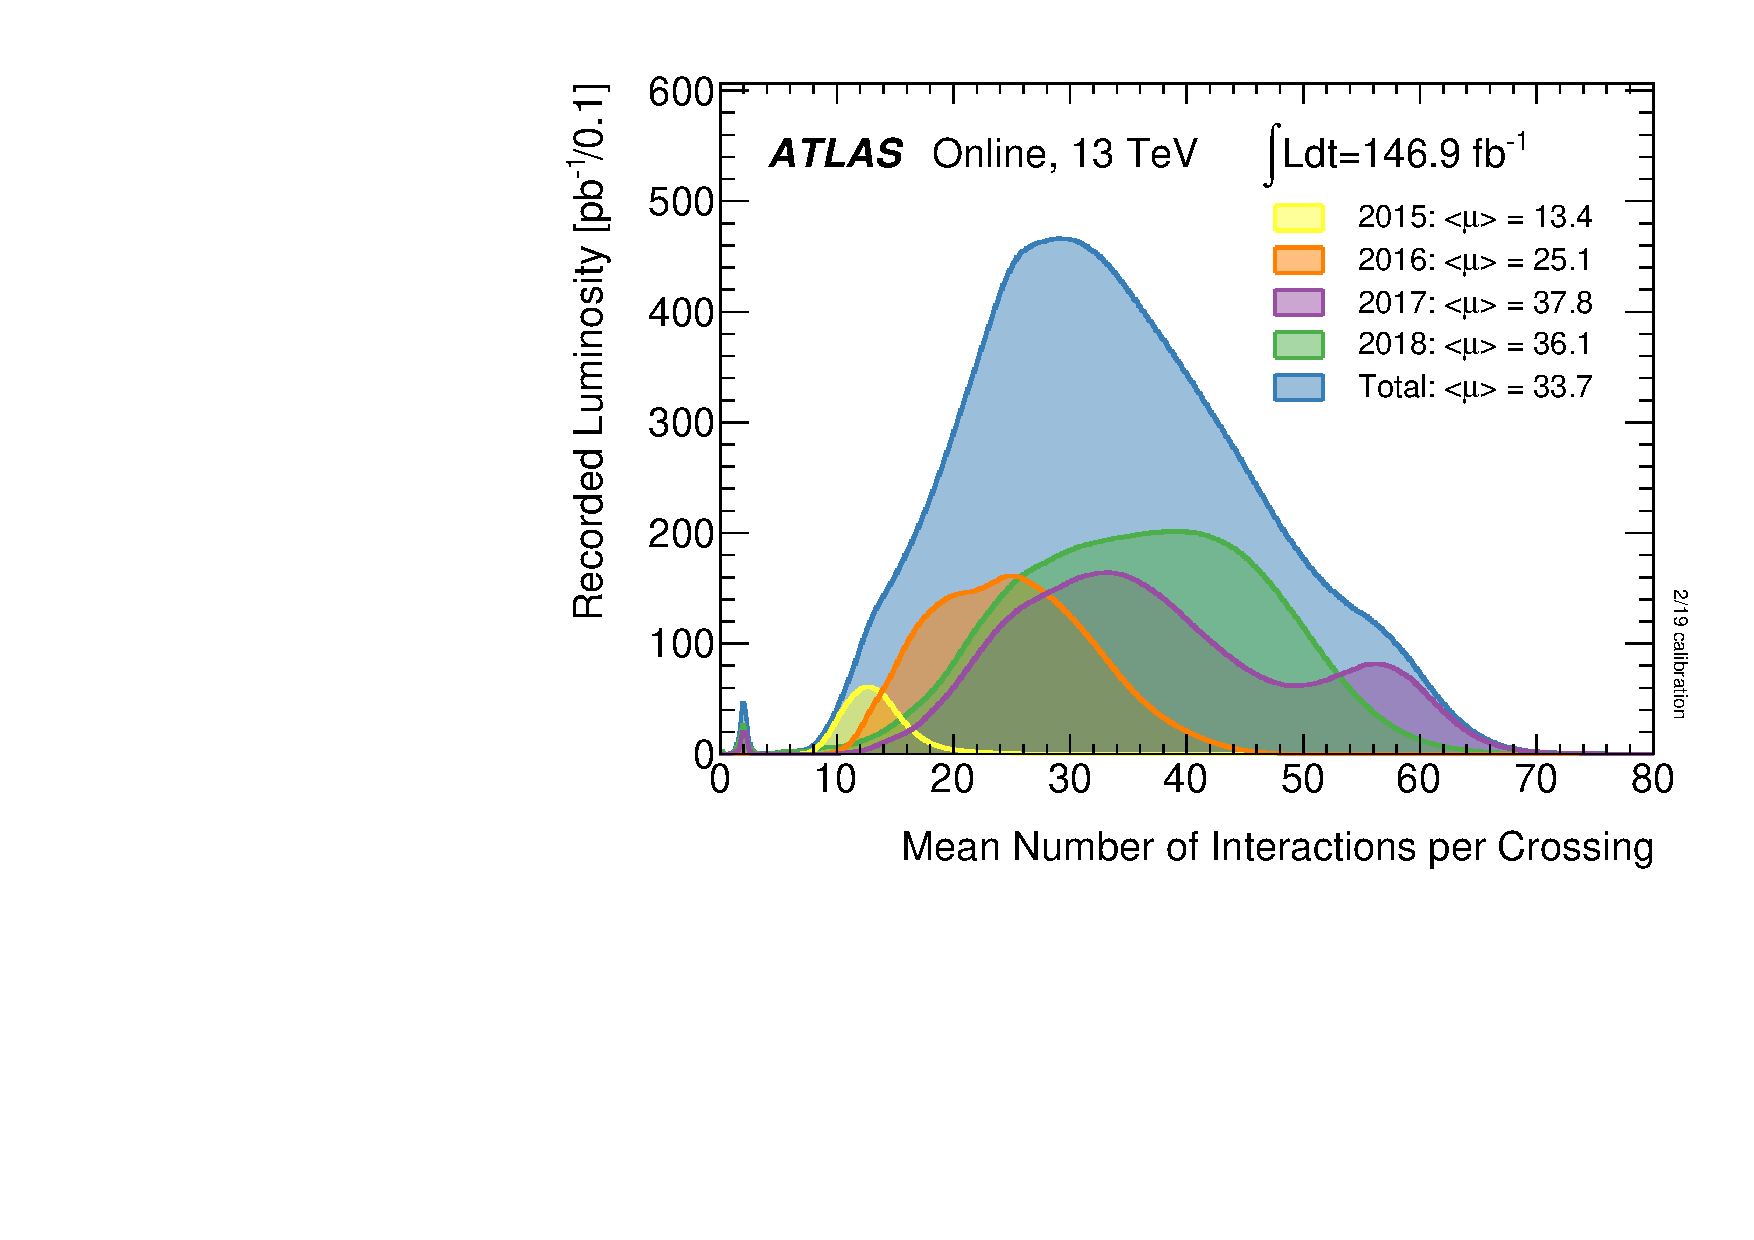
\includegraphics[width=\smallfigwidth]{Figures/LHC/PileUp_2015_2018.pdf}
  \caption[Pile-up distributions.]
  {The pile-up, $\mu$, is the mean number of collisions per bunch crossing. Shown is the \unit{13}{\TeV} are the pile-up distributions from 2015-2018, where each distribution is luminosity weighted.}
  \label{fig:Pileup}
\end{figure}

\section{The ATLAS detector}\label{sec:ATLAS}

Measuring forty-six meters in length, twenty five meters in height and width, and weighing in at a hulking seven thousand tons, the ATLAS (A-Toroidal-LHC-ApparatuS) detector is the Mount Everest of particle detectors. Built with a cylindrical and symmetric structure around the beam pipe, it's detection region covers nearly the entirety of the $4\pi$ solid angle of the collision point. \ATLAS is a general purpose detector, and combines a multitude of detector technologies to conduct searches for new phenomena, and to make high-precision measurements of the Standard Model.

The right-handed coordinate system used by the ATLAS detector, and also very commonly in particle physics, is illustrated in figure \ref{fig:atlascoordinate}. The $z$-axis is parallel to the beam pipe, the $y$-axis points vertically to the sky, and the $x$-axis points to the centre of the \LHC ring. The $xy$-plane is often referred to as the transverse plane, and the frequently encountered variables $p_T$ and $E_T$ refer to the momentum and energy in the transverse direction respectively. The azimuthal angle in the transverse plane is denoted as $\phi$, and polar angle $\theta$ denotes the angle offset from the beam pipe. Another commonly used coordinate is the rapidity, $y$, of an object:
\begin{equation}
    y=\dfrac{1}{2}\ln\dfrac{E+p_Z}{E-p_Z},
\end{equation}
where $E$ is the object's energy and $p_Z$ is the momentum in the $z$-direction, or pseudorapidity $\eta$ in the massless limit:
\begin{equation}
    \eta=-\ln\tan \dfrac{\theta}{2}.
\end{equation}
Both rapidity and pseudorapidity are more commonly used than polar angle $\theta$. The separation of two detected objects, $\Delta R$, is given by
\begin{equation}
    \Delta R=\sqrt{\Delta\eta^2+\Delta\phi^2}.
\end{equation}

\begin{figure}
    \centering
    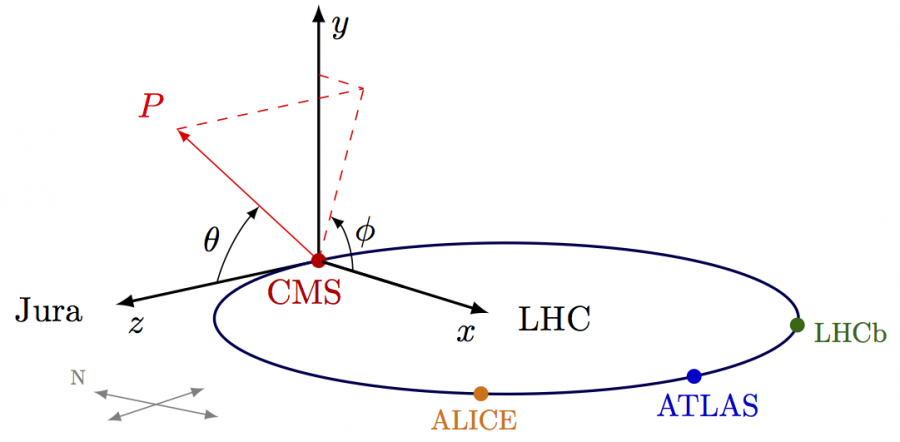
\includegraphics[width=\smallfigwidth]{Figures/LHC/cms_coordinate_system.png}
    \caption{Spherical coordinate system used at the LHC.}
    \todo[inline]{Change to ATLAS}
    \label{fig:atlascoordinate}
\end{figure}

The rest of this section will review the three sub-detectors of \ATLAS - the Inner Detector, the Calorimeter, and the Muon Spectrometer - as well as the Magnet System. A cross-sectional diagram illustrating the sub-detector systems is shown in Figure \ref{fig:atlasdetector}. The sub-detectors are made up on a concentric barrels that wrap around the beam pipe, and circular endcaps placed at either end of the barrels. The barrels are designed to detect the particles that travel through the central $|\eta|$ region, and the endcaps broadens the angular coverage for particles whose trajectories run close to parallel to the beam. 

\begin{figure}
    \centering
    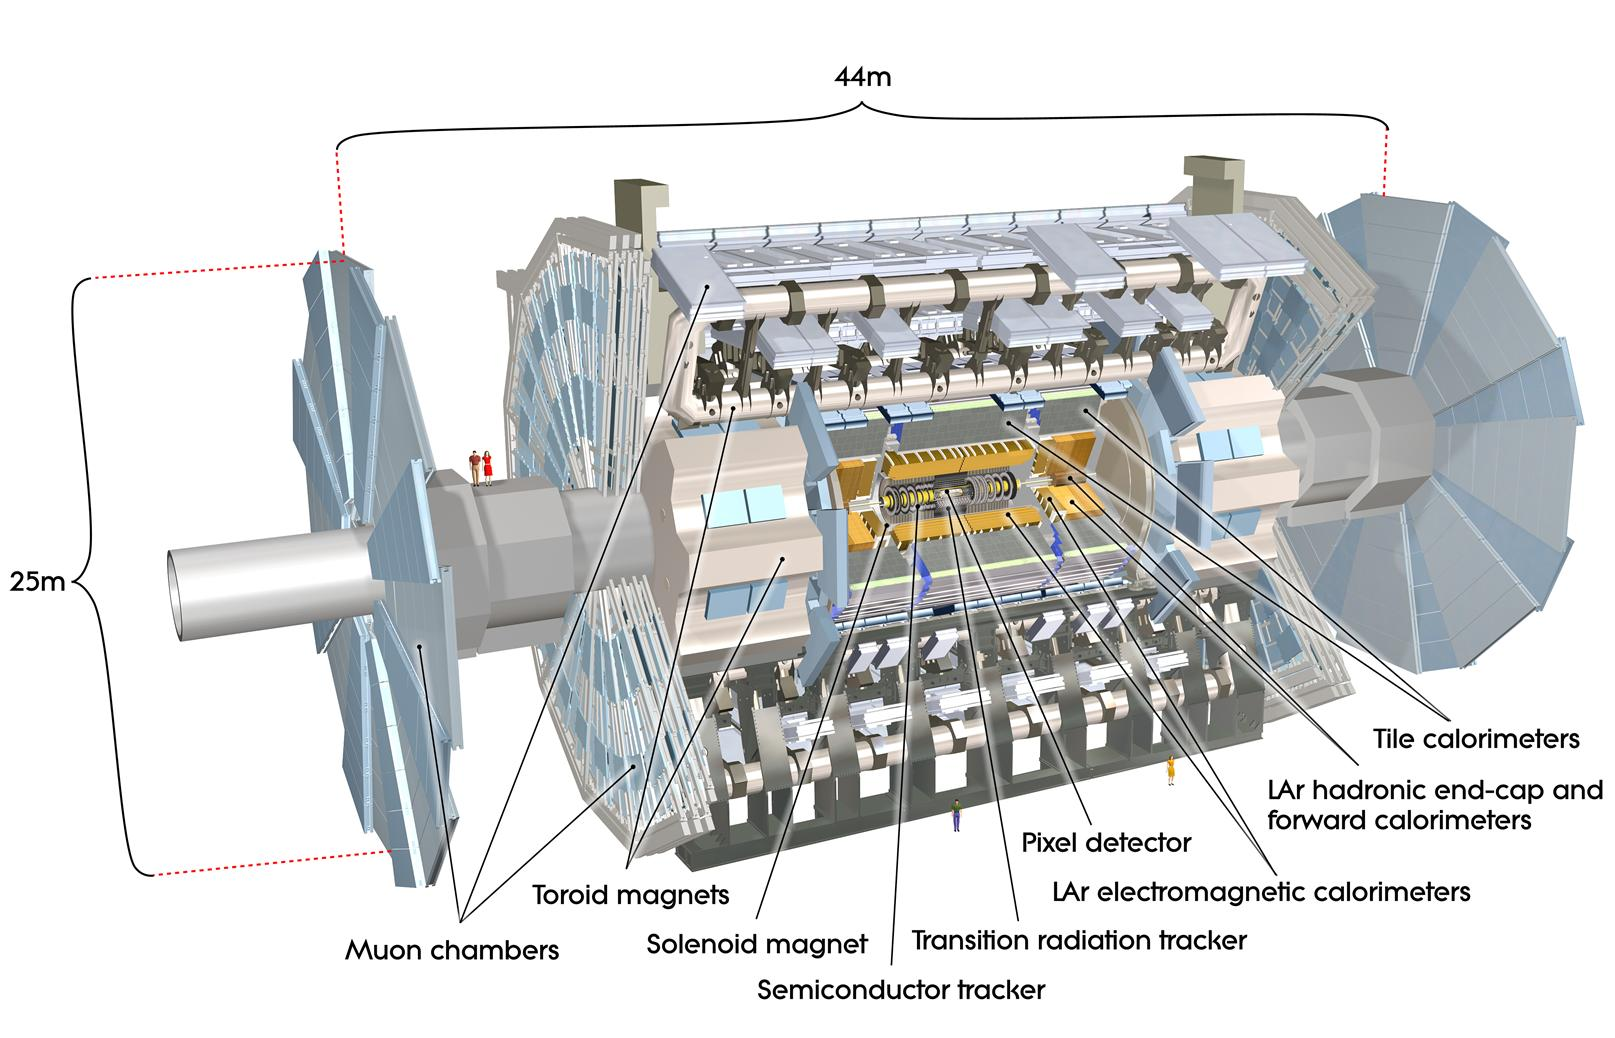
\includegraphics[width=\smallfigwidth]{Figures/LHC/ATLASDetector.jpg}
    \caption{The \ATLAS detector and its sub-componenets.}
    \label{fig:atlasdetector}
\end{figure}

\subsection{The Muon Spectrometer}
The outermost layer of the \ATLAS detector system is the Muon Spectrometer, which as the name suggests, is designed to provide efficient, high-resolution measurements of muons' trajectory and momenta. Installing this tracking system wrapping around the other sub-detectors gives muons a very distinctive detector signature, leading to a high purity and efficiency in their reconstruction. Figure \ref{fig:muonspectrometer} shows the layout of the muon system, which consists of four gaseous tracking chambers installed between the eight coils of the barrel toroidal magnetic system, as well as before and after the toroid magnets of the endcaps. Two of these are precision tracking chambers made for precision momentum measurements, and the other two act as an efficient trigger system fast response \cite{PALESTINI2003337}. 

\begin{itemize}
    \item Monitored Drift Tubes (MDT): To provide precision coordinate measurements in the bending plane of the the muon spectrometer, Monitored Drift Tube (MDT) chambers are installed over the full pseudorapidity range $|\eta| < 2.7$. Each MDT component consists of a 3 cm diameter pressurised aluminium drift tube filled with 93\% argon and 7\% carbon dioxide gas at three bar \cite{LEVIN2008347}. As a muon passes through a drift tube, ionisation electrons drift towards the centre where a wire stretches through the longitudinal axis. 
    \item Cathode Strip Chambers (CSC): The number of MDTs is reduced in the forward region $2.0 < |\eta| < 2.7$, where particle flux is twenty times higher than the average in the rest of the MS. Here, Cathode-Strip Chambers (CSC), momentum measurement. The CSC are multi-wire proportional chambers, with the cathode segmented into strips, and the direction of the strip is perpendicular to one of the wires. This allows for two independent measurements of the muon: one for the ionisation electrons that are collected at the wire, the other one from the induced signal collected at the strips. \change[]{Reword, this is copy pasted.}
    \item Resistive Plate Chambers (RPC): Installed in the barrel region, these chambers provides fast tracking in the $\eta<1.05$ region. Each chamber is made up of two gaseous volumes, Bakelite plates, and read-out electronics \cite{PALESTINI2003337}. 
    \item Thin Gap Chambers (TGC): The Thin Gap Chambers are multiwire proportional chambers characterized by a wire-to-cathode distance smaller than the distance between the wires (1.4 mm and 1.8 mm respectively) – hence the name. This feature in combination with a highly-quenching gas mixture of n-pentane and CO2 allows fast and safe operation at high particle flux. The signal read from the wires provides a bending direction position measurement with a few-mm accuracy. Copper strips separated from a graphite cathode plane by a flameresistant material layer provide an azimuthal measurement with a similar accuracy. Each end-cap comprises nine layers of TGC gas volumes in total – a doublet in each TGCI, TGC2 and TGC3, and a triplet in TGC1 for better background rejection \change[]{copy pasted, change}.
\end{itemize}

\begin{figure}
    \centering
    
\includegraphics[width=\smallfigwidth]{Figures/no-image.png}
    \caption{The Muon Spectrometer}
    \label{fig:muonspectrometer}
\end{figure}

\subsection{The Calorimeters}
The calorimeters allows the measurement of the energies of particles which
pass through the detector. The \ATLAS calorimeters consist of two separate
subcomponents: the Electromagnetic Calorimeter and the Hadronic
Calorimeter.

\subsubsection{The Electromagnetic Calorimeter}
The EM Calorimeter (ECal) is an accordion-shaped structure made up of layers of
lead and stainless steel. In between them is liquid argon cooled to -185
degrees Celsius, and a copper grid immersed inside this liquid. The liquid argon serves as the particle absorber, and the copper grid as the electrode. A particle passing through will interact with the absorber, resulting in a shower of particles. This particle shower moves through the liquid argon and ionises
the atoms. The negative charges are attracted to the copper grid, and from
the amount of charge deposited on the grid it is possible to measure the
energy possessed by the original electron or photon.

\subsubsection{The Hadronic Calorimeter}
The Hadronic Calorimeter (HCal) is designed to measure the energies of hadrons
(neutrons, protons, and mesons) that pass through. It consists of inter-
weaving sheets of steel and plastic scintillator tiles which radiate light with
charged particle exposure. The tiles are placed in the plane perpendicular
to the beam, and different layers are staggered in depth. As a hadron enters the calorimeter, it interacts with the atomic nuclei of the steel sheets.
This ultimately results in a shower of particles which enter the scintillator.
Fibres carry the light from the scintillator to devices that then convert the
light into current. It is then possible to measure the energy of the hadron
that entered the calorimeter.

\subsection{The Inner Detectors} \label{ssec:ATLASID}
The Inner Detector (ID) is able to measure the momentum of charged particles passing through it. The trajectories of the charged particles as they cross through are curved by a superconducting solenoid magnet\todo{of what strength?}. The direction of curvature indicates the particle's charge, while the degree of curvature indicates momentum. The Inner Detector is the smallest component of ATLAS, stretching out to a radius of only 1.15 meters, with a total length of 7 meters. The barrel arrangement consists of concentric cylinders wrapped around the beam axis, and the end-cap components are attached as disks normal to the beam axis. The inner detector has three main components: the Pixel Detector, the Semiconductor Tracker (SCT), and the Transition Radiation Tracker (TRT).

\subsubsection{Pixel Detector}

The Pixel Detector is the innermost part of the Inner Detector. It is the part of ATLAS that is closest to the interaction point where particles collide. It was designed with extremely high granularity in mind in order to accurately resolve primary and secondary vertices, determine impact parameter resolution, and identify short-lived particles such as b-hadrons and tau leptons. Prior to Run 2, the pixel detector consisted of three concentric layers in the barrel, and three disks in the end-cap regions. During the long shutdown prior to Run 2, an additional layer called the Insertable B-layer (IBL) \cite{Capeans:1291633} was added to the Pixel Detector closest to the beam pipe, making a total of four layers. The pixel detector are made up of sensor modules, each consisting of 46,080 active silicon pixels measuring 50 micrometers in width ($\phi$ direction) and 400 micrometers in length ($z$ direction). Each module consist of the active sensor medium (in this case silicon), and front-end electronics for readout. In total, the pixel detector hosts an astonishing eighty million readout channels. All together, the pixel detector achieves a resolution of \unit{10}{\micro\meter} in the $\phi$-direction and \unit{115}{\micro\meter} in the $z$-direction \todo{Check these numbers and cite}.

\subsubsection{Semi-conductor tracker}

The second layer of the inner detector is the SemiConductor Tracker (SCT), made up of two-sided modules of silicon microstrip sensors arranged back to back and tilted by a stereo angle of 40 mrad \cite{AHMAD200798}. It wraps around around the pixel detector and has in total 4088 modules, assembled in four cylindrical layers in the barrel region, and two end-caps containing nine disks each \cite{CERN-LHCC-2017-005}. The stereo angle enables the module to provide information about where along the strip the hit occurred. This is turn gives resolution in the z-plane in the barrels, and in R along the endcaps. The spatial resolution of the detector is \unit{17}{\mu\meter} in $R-\phi$ coordinate and \unit{580}{\mu\meter} in the $z$ coordinate in the barrel ($R$ in the endcaps) \cite{Abdesselam:974073}. In total the SCT hosts 4088 modules, assembled in four cylindrical layers in the barrel region, and two end-caps containing nine disks each \cite{CERN-LHCC-2017-005}. 

\subsubsection{Transition Radiation Tracker}

The third and outermost layer of the inner detector is the Transition Radiation Tracker (TRT). Unlike the ID and the SCT, it uses a straw drift tube technology, and exploits transition radiation emission for additional particle identification. Each module consists of 4 millimetre diameter straw tubes filled with xenon, carbon dioxide, and oxygen (70\%, 27\%, and 3\%)\cite{Vogel:1537991} bundled together. In order to collect charge from ionisation, a tungsten wire extends axially through the centre of each tube. In the barrel the drift tubes run parallel with the beam axis, and in the endcaps they run radially. In total there are 351,000 readout channels, and the resulting position resolution is weaker than the Pixel Detector or the SCT. The TRT is only capable of performing measurements in the $R-\phi$ coordinate, with a resolution of \unit{170}{\mu\meter} \cite{missing}. Despite the lower resolution and the lack of sensitivity in the z coordinate, the hits in the TRT contribute significantly to momentum resolution due to the a larger number of measurements and an extended measured track length. Furthermore, the barrel straws are inter-weaved in a matrix of polypropylene fibres, and the endcap disks are wedged in between polypropylene foils, creating numerous material boundaries. As highly relativistic particles pass through the boundaries they emit transition radiation photons; predominantly in the X-ray energy regime \cite{Ginzburg_1996}. These photons are absorbed by the gas mixture inside the tubes, and yield higher signal amplitudes than the signal of hits from minimum-ionizing particles. The energy of the transition radiation photon is strictly proportional to the relativistic factor $\gamma=E/m$ of the incident particle. For a given momentum, it is much higher for electrons than it is for pions or muons, a useful difference that is exploited for particle identification.